\chapter{Développement d'outils logiciel et matériel d'investigation}
\label{chap:2}
\section{Méthode de modélisation au niveau système}

% Need to simulate from source to input for soft-failure analysis
Un environnement de test ESD est composé d'éléments récurrents tels que des sources DC, des oscilloscopes, des générateurs de stress et des cartes électroniques interconnectés par des câbles et des fils.
Les cartes électroniques embarquent différents types de composants, tels que des composants passifs, des protections ESD et des circuits intégrés.
Afin de simuler le comportement de tous ces éléments pendant une décharge ESD, une méthodologie de modélisation au niveau système est proposée.
Elle permet une simulation précise jusqu'à l'entrée d'un circuit intégré en fonctionnement.
L'objectif de la méthode proposée est tout d'abord de construire une librairie des éléments les plus courants, puis d'assembler ces éléments ensembles pour former le modèle complet du système à étudier.

% Cables and delays identified as important for esd sims - because of similar order of magnitude
Les câbles sont des éléments importants mais parfois négligés dans les simulations ESD.
Ils introduisent des délais de propagation non négligeables par rapport à la durée d'un ESD.
Pour ordre de grandeur, un câble coaxial 50\textOmega{} possède une constante de propagation d'environ 5 ns/m.
En comparaison, un ESD dure entre une dizaine et plusieurs centaines de nanosecondes, ce qui est globalement proche du même ordre de grandeur.
Les câbles sont avant tout des lignes de transmission, dont l'analyse théorique fut faite par J. Maxwell, L. Kelvin et O. Heaviside et énormément étudiées par la suite dans la littérature \cite{branin-tl-ref, hf-coax,lossy-tl,emc-analysis-tl}.

% Distributed model
Le modèle le plus populaire de ligne est basé sur des éléments distribués.
Concrètement, c'est une suite réseaux L-C tels que la Fig. \ref{fig:dis-line-model}.
Les valeurs de chaque élément sont calculées à partir des propriétés du câble et de la précision requise pour la simulation.

\begin{figure}[!h]
  \centering
  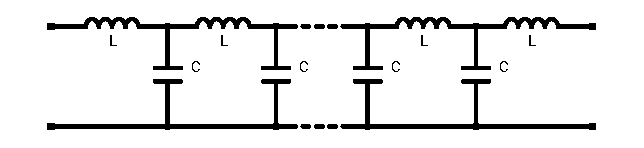
\includegraphics[width=0.7\textwidth]{src/1/figures/lc_ladder.pdf}
  \caption{Modèle de ligne de transmission LC distribué}
  \label{fig:dis-line-model}
\end{figure}

% Perks and disavantages
Malgré sa très large adoption, ce modèle présente de sérieux inconvénients.
En particulier, ce modèle nécessite un très grand nombre d'éléments pour avoir une précision correcte de simulation de câbles longs tels que le câble de 10m d'un TLP.
Pour une même précision, le nombre d'éléments est proportionnel à la longueur du câble, ce qui augmente considérablement les temps de simulation.
Pour augmenter la bande passante du modèle, le nombre d'éléments doit également être augmenté.
La combinaison des deux résulte en des temps de simulation très longs.

% Behavioral model
Le modèle à deux ports décrit par H. Branin \cite{branin-tl-ref} est une alternative bien plus performante au modèle distribué.
Il décrit très efficacement et avec une très grande précision le comportement d'une ligne de transmission.
La bande passante n'est pas limité, et le temps de simulation est indépendant de la longueur du câble.
Le modèle est constitué de deux sources de tension contrôlées en tension et deux résistances (Fig. \ref{fig:beh-line-model}).

\begin{figure}[!h]
  \centering
  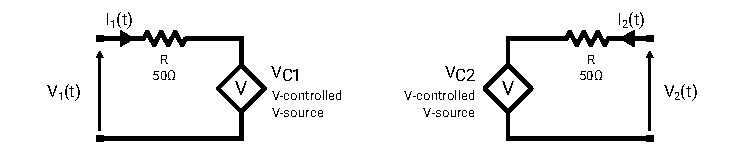
\includegraphics[width=\textwidth]{src/1/figures/behavioral_line_model.pdf}
  \caption{Modèle comportemental d'une ligne de transmission sans pertes}
  \label{fig:beh-line-model}
\end{figure}

Les équations définissant le comportement des sources de tension sont données dans le document final.
Elles décrivent un système où tension et courant à chaque port sont la superposition d'une onde se propageant dans un sens et d'une seconde dans l'autre sens.

% Model other devices
La modélisation d'autres éléments importants tels que les composants passifs et les protections ESD est détaillé dans le document complet.

% Illustrate the method with a practical case
Pour illustrer l'application de la méthode de modélisation, elle est appliquée sur un banc TLP du laboratoire de NXP Toulouse.
C'est un bon cas d'étude afin d'utiliser la méthode, car ce banc est très largement utilisé pour l'investigation.
Pour démontrer sa précision, le modèle est vérifié par comparaison avec de multiples mesures, sous différentes charges et amplitudes.

\begin{figure}[!h]
  \centering
  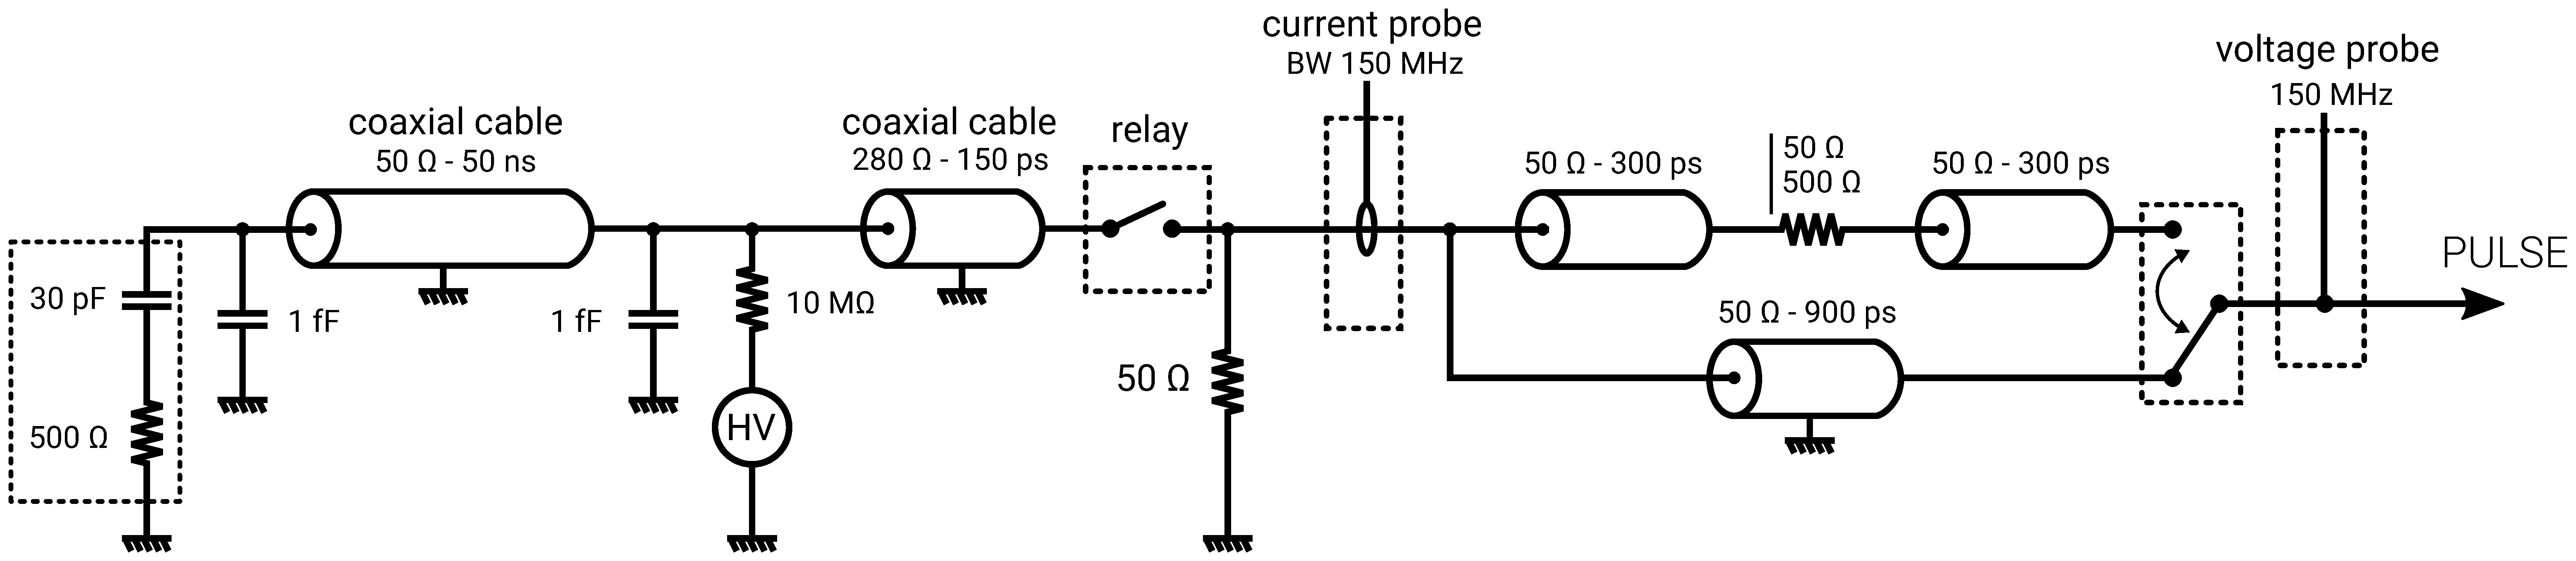
\includegraphics[width=\textwidth]{src/1/figures/complete_nxp_tlp_model.pdf}
  \caption{Modèle complet du générateur TLP du laboratoire NXP Toulouse}
  \label{fig:complete-tlp-model}
\end{figure}

% Explain how the model, how it was constructed
Le modèle complet de TLP est donné en Fig. \ref{fig:complete-tlp-model}.
Il reproduit l'architecture du TLP du laboratoire en utilisant des modèles de la librairie pour chaque élément.

% Detail a first comparison with 25 ohms
Une première comparaison entre une mesure et simulation est donnée en Fig. \ref{fig:comparison-tlp-load}.
Avec une charge de 25\textOmega{} et une tension de charge de 500 V, un courant de 4.5 A et une tension de 125 mV sont relevés sur le second plateau de la courbe.
Le rapport de ces deux valeurs corresponds bien à 25\textOmega{} comme attendu.
Jusqu'à 220 ns, les deux courbes se ressemblent fortement.
Après 220ns, des différences apparaissent, supposées dues aux erreurs de modélisations.
La plupart des simulations ESD restent intéressantes pendant la partie principale de la décharge jusqu'à 120 ns et ces erreurs sont donc négligeables.

\begin{figure}[!h]
  \centering
  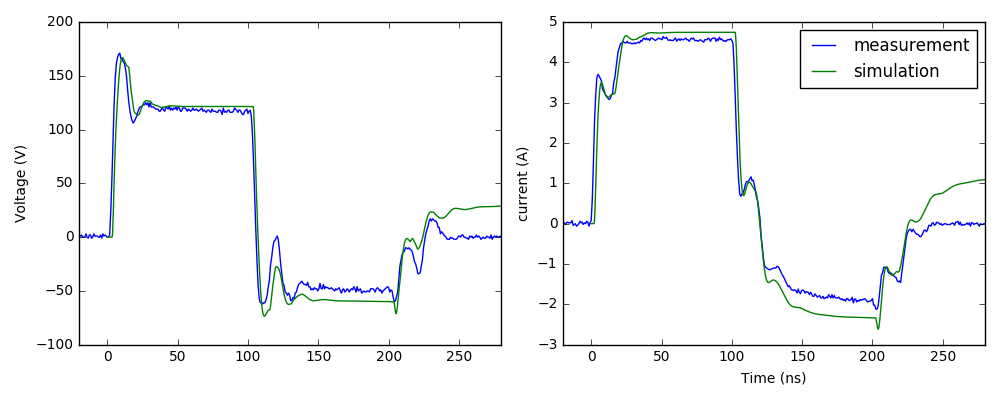
\includegraphics[width=\textwidth]{src/1/figures/tlp_comparison_R25_500V.png}
  \caption{Comparaison des courbes temporelles de tension et courant avec une  tension de charge 500 V sous 25\textOmega{}}
  \label{fig:comparison-tlp-load}
\end{figure}

% More validations in Annex
Les autres validations sont données dans le document complet, et présentent des niveaux de corrélations aussi proches.
Le modèle fonctionne correctement et reproduit les mesures, prouvant sa validité.

\section{Développement d'un générateur TLP modifié}

% TLP is a great tool for esd analysis
Le TLP est capable de générer des impulsions très bien contrôlées et reproductibles.
L'utilisation des pistolets ESD reste obligatoire pour la qualification de produits.
La forme d'onde la plus répandue est celle définie dans la spécification HMM \cite{hmm} et les standards IEC 61000-4-2 \cite{iec61000-4-2} et ISO 10605 standard \cite{iso10605}.
Ensemble, ils couvrent une très large plage d'applications, dans les domaines grand-public, automobile et industriel.
Pour combiner les avantages d'un TLP avec ceux d'une décharge HMM, un générateur TLP peut être modifié pour produire cette impulsion HMM.
Cette approche a été explorée par le passé par E. Grund \cite{iec61000-tlp} et Y. Cao \cite{tlp-based-hmm}.
Néanmoins, leurs techniques présentent quelques inconvénients tels que une tendance large à créer des oscillations, comme démontré dans le document complet.

Le générateur proposé ici est dénommé TLP-HMM.
Le TLP-HMM requiert deux modules additionnels à connecter à chaque extrémité d'un TLP standard 100 ns.
Ils sont nommés \textit{absorber} et \textit{shaping filter} (Fig. \ref{fig:tlp_hmm_architecture}).
Le principe du TLP-HMM est de re-router une portion du courant incident dans la masse, de manière à ce que le courant restant prenne la forme de l'onde HMM.
Le fonctionnement de chaque élément est détaillé dans le document final.

\begin{figure}[!h]
  \centering
  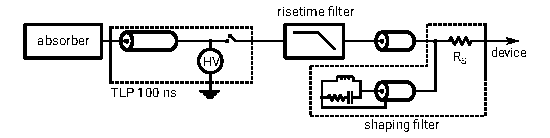
\includegraphics[width=0.9\textwidth]{src/1/figures/beges_tlp_hmm.pdf}
  \caption{architecture du TLP-HMM}
  \label{fig:tlp_hmm_architecture}
\end{figure}

Les courbes simulées et mesurées sur un prototype sont données Fig. \ref{fig:tlp_hmm_waveforms}.
Les courants mesurés à 30 ns et 60 ns sont dans la marge de tolérance de 30\% des standards, et elle est donc valide.

\begin{figure}[!h]
  \centering
  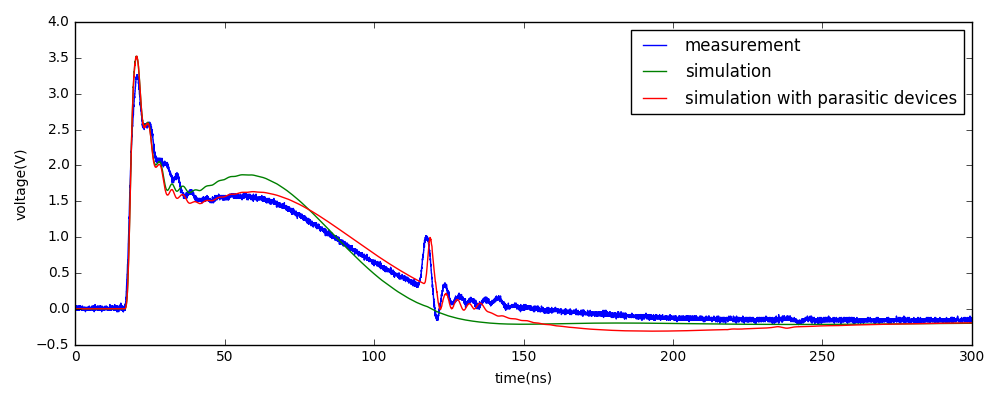
\includegraphics[width=0.95\textwidth]{src/1/figures/tlp_hmm_waveforms.png}
  \caption{Mesure et simulation d'une décharge 250 V TLP-HMM (équivalente 1 kV HMM) sur 2\textOmega{}}
  \label{fig:tlp_hmm_waveforms}
\end{figure}

% Analyse the curve
Globalement, la simulation et la mesure corrèlent bien.
Il y a des différences mineures, notamment entre 40 ns et 150 ns.
Elles sont dues à des éléments parasites non pris en compte durant les simulations, et des corrections sont à apporter au prototype.
L'analyse de ces éléments est fournie dans le document complet.

\section{Méthode de traitement de capteurs de courant on-chip}

% Introduction
Avec une mesure de champ-proche, il est possible de mesurer des cartographies de champ électrique ou magnétique.
Dans ce chapitre deux méthode de reconstruction sont évaluées afin de retrouver des valeurs de courant depuis une cartographie de champ magnétique.
Le capteur de champ proche sur silicium présenté dans le chapitre 4 est utilisé pour obtenir des mesures de courant sur puce.

% What is the output voltage that is measured
La méthode temporelle consiste simplement à intégrer le signal mesuré en y appliquant des facteurs correctifs.
Il est montré dans \cite{near-field-scan} que cette approche est valide.
Le schéma de la méthode de mesure est donnée Fig. \ref{fig:calibration-sensor}.
Une impulsion rectangulaire de 100 ns et 1 V est injectée entre S1 et S2.
La tension V\textsubscript{sensor} est mesurée avec un oscilloscope 2 GHz entre C1 et C2.

\begin{figure}[!h]
  \centering
  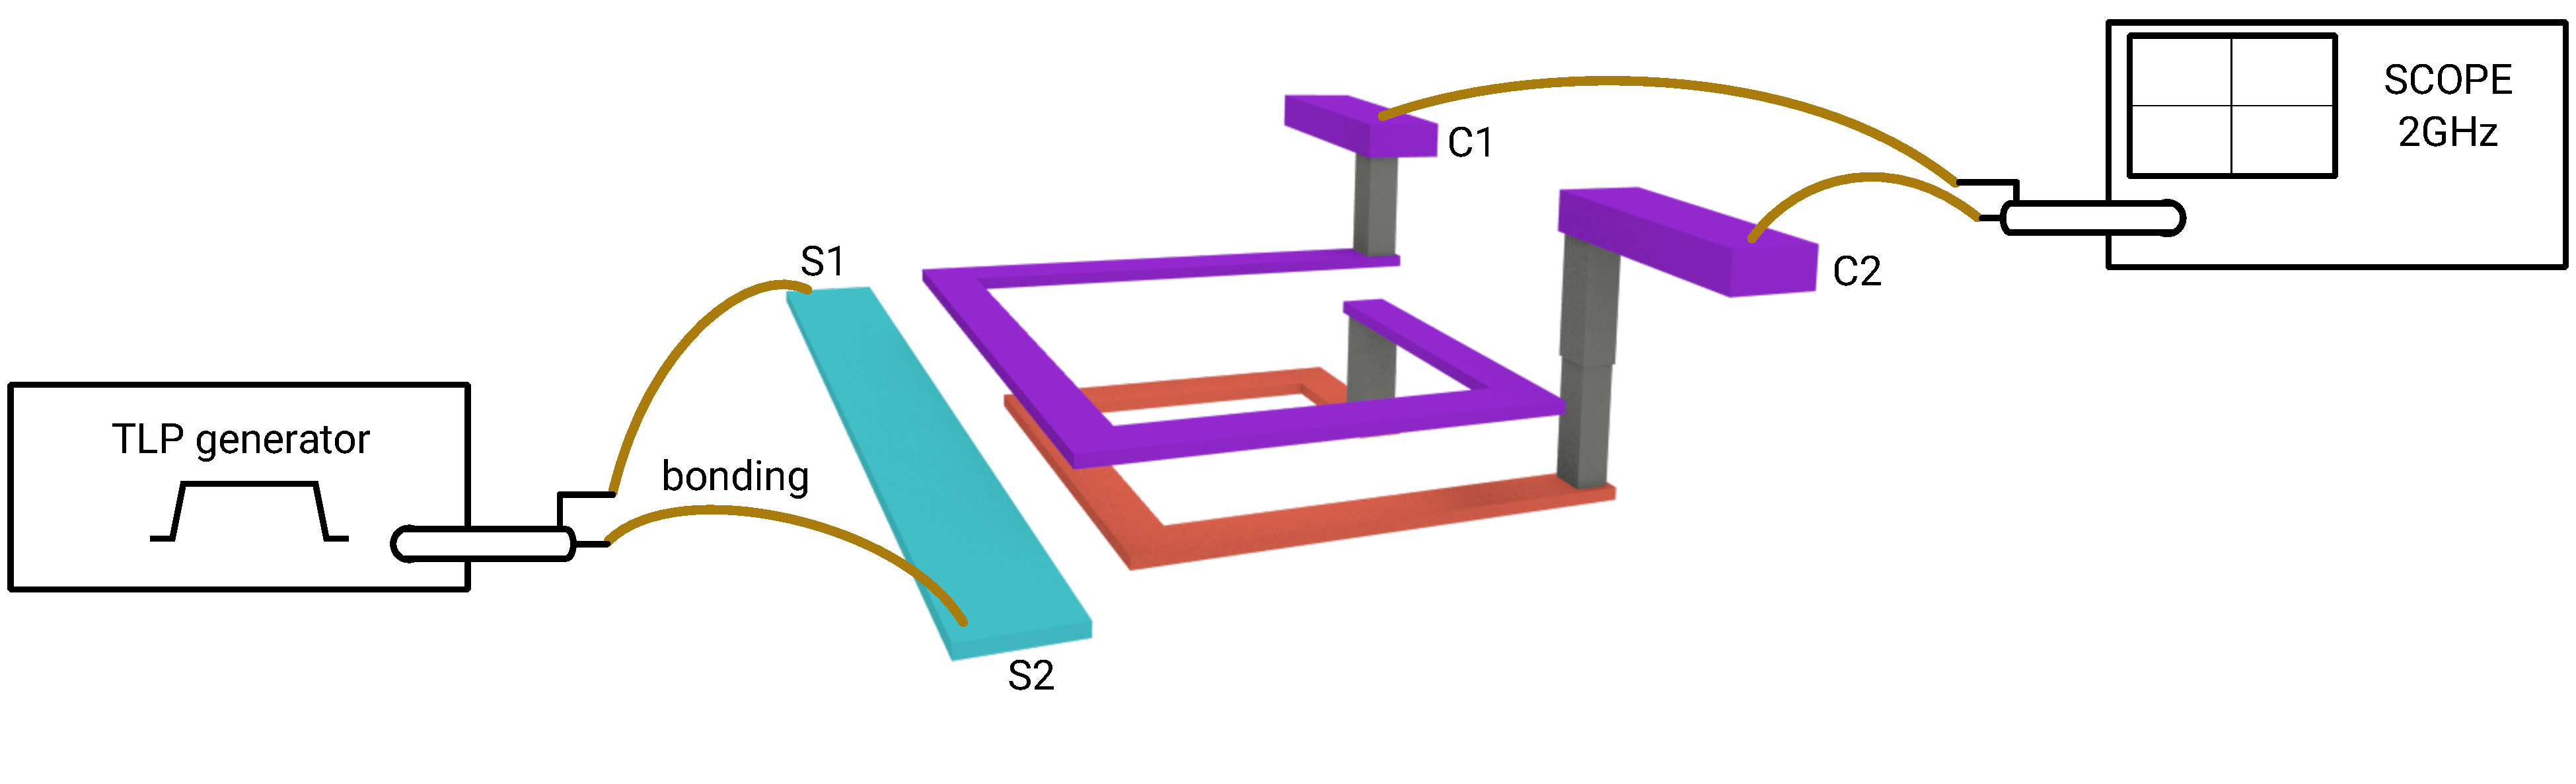
\includegraphics[width=0.9\textwidth]{src/1/figures/sensor_measurement_setup.pdf}
  \caption{Montage de calibration du capteur de courant sur silicium dans le domaine temporel}
  \label{fig:calibration-sensor}
\end{figure}

% Intro & Characterization
La méthode fréquentielle utilise une mesure paramètre-S du capteur pour traiter V\textsubscript{sensor}.
Le montage de calibration est similaire à la méthode temporelle et donnée dans le document final.
Elle est basée sur une utilisation de la réponse fréquentielle du capteur pour corriger les mesures temporelles.

Une comparaison de la courbe originale, de la méthode temporelle, et de la méthode fréquentielle sont fournies Fig. \ref{fig:freq-domain-reconstructed}.
Globalement, les résultats sont similaires en terme de précision.
La courbe mesurée est obtenue par reflectométrie, ce qui explique pourquoi elle possède plusieurs plateaux contrairement aux simulations.
De multiples améliorations sont possibles pour les deux méthodes, et des pistes sont proposées dans le document final.

\begin{figure}[!h]
  \centering
  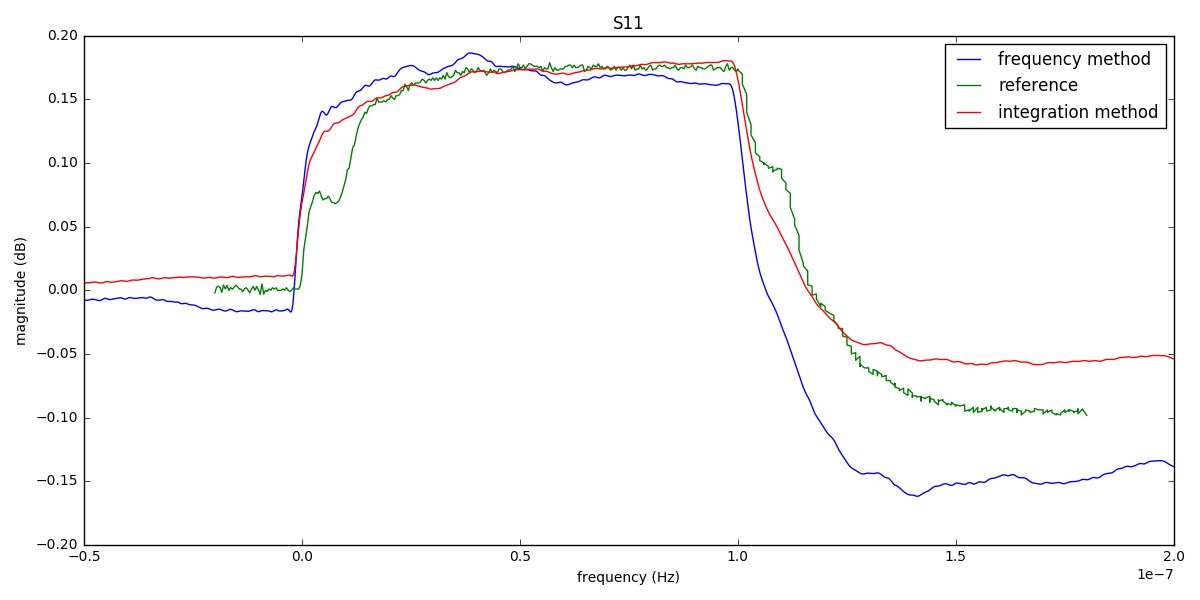
\includegraphics[width=0.9\textwidth]{src/1/figures/final_comparison_reconstructions.png}
  \caption{Courant de référence, reconstruction par méthode temporelle et fréquentielle}
  \label{fig:freq-domain-reconstructed}
\end{figure}
